\section{Propylene}

\subsection{Overview}
%------------------------------
\begin{frame}{Propylene architecture}
  %%
  Propylene is made of several stand-alone modules:
  %%
  \begin{figure}[!h]
    \begin{center}
      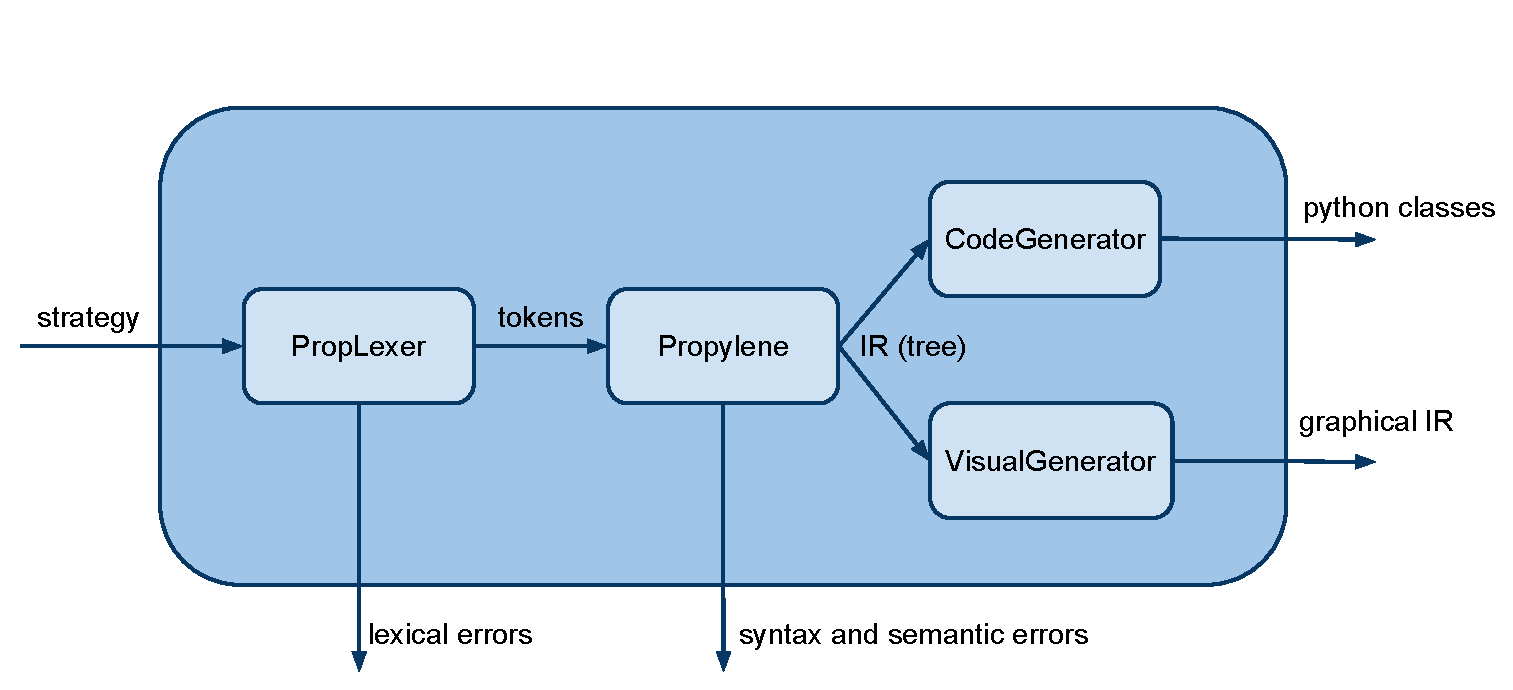
\includegraphics[width=300pt]{img/propylene.pdf}
    \end{center}
  \end{figure}
  %%
  Internally, it implements a \green{symbol table}.
  %%
\end{frame}


\subsection{AST}
%------------------------------
\begin{frame}{AST}  
  %
  %% \begin{itemize}
  %% \item Info concerning AST generation and traversal
  %%   \N
  %% \item Could contain some notes on Node hierarchy or Visitor
  %%   \N
  %% \item More...
  %%   \N
  %% \item AST Graphics here??
    
  %% \end{itemize}
  %
%
\N\N
\end{frame}



\subsection{Error Handling}
%------------------------------
\begin{frame}[fragile]{Syntax Errors}
  %
  \begin{itemize}
    \item \navy{Propylene} attempts to recover from erroneous input 
    by using its error rules
\n
    \item When the encountered syntax errors exceed a threshold, 
    the parser stop
\n
    \item The user will be notified with info related to all errors
    
  \end{itemize}
  %
\N
%%
  \begin{exampleblock}{Error Messages Example}
\begin{verbatim}
Line 14: Syntax error - unexpected token `)'
Line 14: Illegal Triggering Event
Line 17: Error detected in the Condition of the plan
Line 96: Error detected in the Body of the plan
\end{verbatim}
  \end{exampleblock}
%%
%
\N\N
\end{frame}


%------------------------------
\begin{frame}[fragile]{Semantic Errors}
  %
  \begin{itemize}
    \item \navy{Propylene} is able to identify two types of semantic errors:
\n
  %
  \begin{enumerate}
    \item Unbounded Variable \\
\n
    %%
    \texttt {
        ( +\tildett deposit\_corns() | ( white\_corn(\_("Y")))) >>\\ 
        \tab [ +\tildett grab\_corn(\_("X")) \#ERROR! ]
            }
    %%
\N
    \item Attitude Type Mismatch \\
\n
    %%
    \texttt {
        ( +\tildett deposit\_corns() ) >>\\ 
            \tab [ +\tildett grab\_corn("c11") \\
            \tab \tab deposit\_corns() \#ERROR! ]
            }
    %%

  \end{enumerate}
  %
\n
  \item In both cases, the parser stops immediately and notifies the user
  about the encountered error
  \end{itemize}
  %
%
\N\N
\end{frame}


\subsection{Graphics}
%------------------------------
\begin{frame}{Graphics}
  %
  \begin{itemize}
    \item Tree graphics, diagrams
\N
    \item final remarks
%\N
%    \item 
%\N
%    \item
% 
  \end{itemize}
  %
%
\N\N
\end{frame}







%\subsection{}
%%------------------------------
%\begin{frame}{}
%  %
%  \begin{itemize}
%    \item
%\N
%    \item
%\N
%    \item 
%\N
%    \item
% 
%  \end{itemize}
%  %
%%
%\N\N
%\end{frame}


